% !TeX root = ../.tex
\begin{frame}[t]
  \frametitle{เนคเทคกับ FOSS}

  \begin{columns}

    \column[c]{0.6\textwidth}
    \textbf{ในอดีต}
    \begin{itemize}
      \item ห้องปฏิบัติการโอเพ่นซอร์ส
      \item ลินุกซ์ทะเล (LinuxTLE)
      \item ลินุกซ์ซีส (LinuxSIS)
      \item ลินุกซ์เพื่อคอมพิวเตอร์ราคาประหยัด(Computer ICT)
      \item ลินุกซ์เพื่อผู้ประกอบการภายในประเทศ (Ecolonux)
      \item ออฟฟิซทะเล (OfficeTLE)
    \end{itemize}

    \column{0.4\textwidth}
    \begin{center}
      
\includegraphics[width=.4\linewidth]{images/linuxtle.png}

      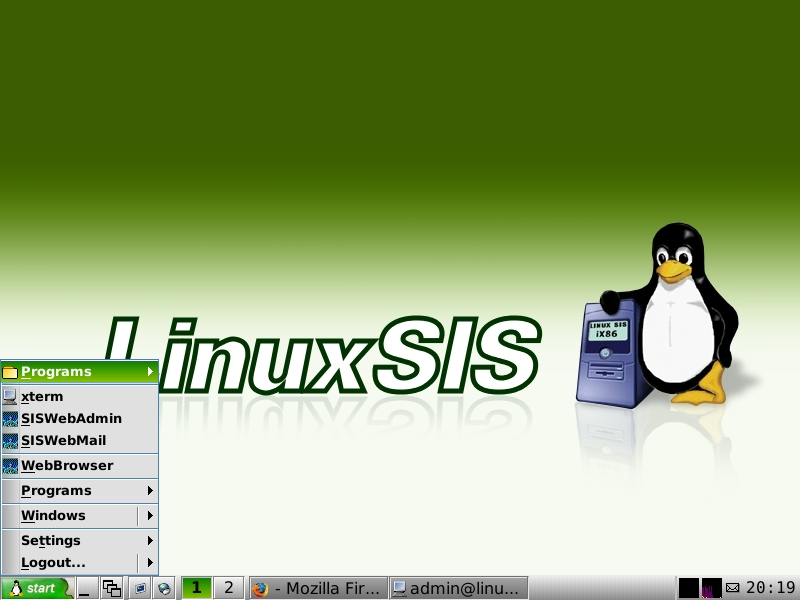
\includegraphics[width=.5\linewidth]{images/linuxsis.jpg}
    \end{center}
  \end{columns}
\end{frame}